\section{Galerkin有限元}
\label{sec:pdenum-galerkin}

差分方法直接逼近导数，要求解有足够多的导数，网格也最好是规则的。第~\ref{chap:elliptic-equations}章的弱形式提供了另一个出发点：方程只需对一族测试函数成立，一阶导数就够了。于是可以换一个问法，不再逼近导数，而是在一个有限维的函数空间里找最好的近似。

这里只讨论二阶椭圆问题。一般泛函的Ritz思想可参考\BookChapterRef{chap:functional-optimization-variation}{卷五第29章“泛函优化”}，本节着重处理边界条件、局部基函数和方程误差。

\subsection{离散弱问题}
\label{sec:pdenum-weak-galerkin}

\paragraph{把试探空间换成有限维}
回忆第~\ref{chap:elliptic-equations}章的抽象形式。设$V$是Hilbert空间，对齐次Dirichlet问题是$H^1_0(\Omega)$；$a$是$V$上的双线性型，$\ell$是$V$上的有界线性泛函。弱问题是求$u\in V$，使
\begin{equation}
 a(u,v)=\ell(v)\qquad\text{对所有}\ v\in V .
 \label{eq:pdenum-weak}
\end{equation}
对问题$-\Delta u=f$，两个对象分别是
\[
 a(u,v)=\int_\Omega\nabla u\cdot\nabla v\,\mathrm{d}\bm{x},\qquad \ell(v)=\int_\Omega fv\,\mathrm{d}\bm{x}.
\]

式~\eqref{eq:pdenum-weak}要对无穷多个$v$成立，未知量$u$也在无穷维空间里。Galerkin的办法是同时限制两者：取有限维子空间$V_h\subset V$，把试探函数和测试函数都取在$V_h$中。

\begin{definition}[Galerkin方程]
 \label{def:pdenum-galerkin}
 设$V_h\subset V$是有限维子空间。求$u_h\in V_h$，使
 \begin{equation}
  a(u_h,v_h)=\ell(v_h)\qquad\text{对所有}\ v_h\in V_h .
  \label{eq:pdenum-galerkin}
 \end{equation}
 $V_h\subset V$这个包含关系称为\term{协调性}（conformity）。
\end{definition}

取$V_h$的基$\varphi_1,\ldots,\varphi_N$，写$u_h=\sum_jc_j\varphi_j$，并依次取$v_h=\varphi_i$。由双线性，式~\eqref{eq:pdenum-galerkin}等价于线性方程组
\begin{equation}
 \bm{K}\bm{c}=\bm{b},\qquad K_{ij}=a(\varphi_j,\varphi_i),\quad b_i=\ell(\varphi_i).
 \label{eq:pdenum-stiffness-system}
\end{equation}
$\bm{K}$称为\term{刚度矩阵}（stiffness matrix），$\bm{b}$称为\term{载荷向量}（load vector）。

若$a$在$V$上强制，常数为$\alpha$，那么对任意$\bm{c}\ne\bm{0}$，
\[
 \bm{c}^\top\bm{K}\bm{c}=a(u_h,u_h)\geq\alpha\lVert u_h\rVert_V^2>0 .
\]
所以$\bm{K}$可逆，离散解存在且唯一。这里用到$V_h\subset V$：强制性是在整个$V$上成立的，子空间自动继承。这就是协调性的第一个用处。

试探函数和测试函数取同一个空间，并不是唯一的选择，但它有清楚的含义。下面的恒等式是Galerkin方法几乎所有性质的来源。

\begin{theorem}[Galerkin正交性]
 \label{thm:pdenum-galerkin-orthogonality}
 设$V_h\subset V$，$u$满足式~\eqref{eq:pdenum-weak}，$u_h$满足式~\eqref{eq:pdenum-galerkin}，则
 \begin{equation}
  a(u-u_h,v_h)=0\qquad\text{对所有}\ v_h\in V_h .
  \label{eq:pdenum-orthogonality}
 \end{equation}
\end{theorem}

\begin{proof}
 由$V_h\subset V$，可以在式~\eqref{eq:pdenum-weak}中取$v=v_h$，得$a(u,v_h)=\ell(v_h)$。减去式~\eqref{eq:pdenum-galerkin}，由双线性即得结论。
\end{proof}

$a$对称正定时，$a(\cdot,\cdot)$本身是内积，式~\eqref{eq:pdenum-orthogonality}说$u-u_h$与$V_h$正交，也就是说$u_h$是$u$在$V_h$上的$a$-正交投影，图~\ref{fig:pdenum-galerkin-projection}是这幅图景。投影作用在未知的$u$上，算法却不需要知道$u$，因为$a(u,\varphi_i)=\ell(\varphi_i)$已由方程给出。$a$不对称时图景不再是投影，但恒等式仍然成立，下一小节的误差分析只用恒等式。

\begin{BookInlineFigure}
 \centering
 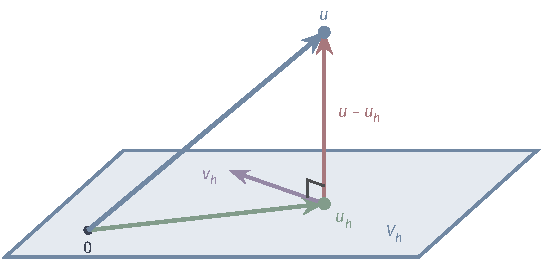
\includegraphics[width=92mm]{figures/06-differential-equations/02-partial-differential-equations/tikz/pdenum-galerkin-projection/figure.pdf}
 \caption{$a$对称正定时的Galerkin方法。真解$u$（蓝）不在有限维子空间$V_h$（浅蓝平面）中，$u_h$（绿）是它关于内积$a(\cdot,\cdot)$的正交投影，误差$u-u_h$（红）与$V_h$中的每个$v_h$（紫）都$a$-正交。}
 \label{fig:pdenum-galerkin-projection}
\end{BookInlineFigure}

\paragraph{非齐次Dirichlet数据}
上面的讨论要求试探函数和测试函数在同一个线性空间里，而边值$u=g\ne0$的函数不构成线性空间。第~\ref{chap:elliptic-equations}章的办法是作边界提升：取任何满足边值的函数$u_g$，令$w=u-u_g$，$w$就是齐次的，方程变成
\begin{equation}
 a(w,v)=\ell(v)-a(u_g,v)\qquad\text{对所有}\ v\in V .
 \label{eq:pdenum-lifted}
\end{equation}

离散时同样要做这一步，右端多出的$-a(u_g,v_h)$不能丢。在节点基下，自然的提升是用边界节点对应的基函数：$u_g=\sum_{p\in\text{边界}}g_p\varphi_p$。把基函数按内部节点I和边界节点B分块，式~\eqref{eq:pdenum-lifted}变成
\begin{equation}
 \bm{K}_{\mathrm{II}}\bm{c}_{\mathrm{I}}=\bm{b}_{\mathrm{I}}-\bm{K}_{\mathrm{IB}}\bm{g}_{\mathrm{B}} .
 \label{eq:pdenum-lifted-system}
\end{equation}

只删除边界节点的行和列，而不把$\bm{K}_{\mathrm{IB}}\bm{g}_{\mathrm{B}}$移到右端，等于把边值改成了零。对例子~\eqref{eq:pdenum-model}，下一小节将算出，正确的系统给出$(0.9571,1.5,1.4571)$，而漏掉这一项给出$(0.7071,1,0.7071)$，那是边值全为零的问题的解，如图~\ref{fig:pdenum-boundary-deletion}所示。

\begin{BookInlineFigure}
 \centering
 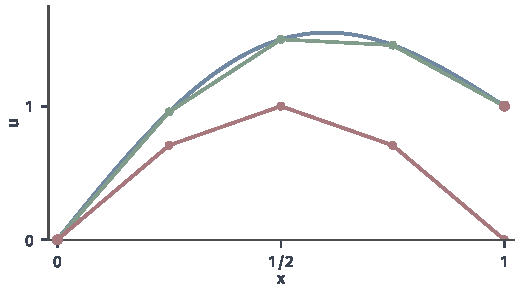
\includegraphics[width=88mm]{figures/06-differential-equations/02-partial-differential-equations/matplotlib/pdenum-boundary-deletion/figure.pdf}
 \caption{$h=1/4$的有限元解。蓝线是真解，红色大点是边值。绿线按式~\eqref{eq:pdenum-lifted-system}处理，节点值落在真解上。红线只删除了边界行和列，右端没有边值的贡献，解的右端回到了$0$。}
 \label{fig:pdenum-boundary-deletion}
\end{BookInlineFigure}

Neumann和Robin条件与此不同。它们是自然边界条件，在弱形式中通过$\ell$和$a$的边界项进入，不需要提升。

\subsection{基函数与组装}
\label{sec:pdenum-assembly}

\paragraph{主要思想}
基函数的选择决定矩阵的结构。若每个$\varphi_i$只在一小块区域上非零，那么$K_{ij}$只在$\varphi_i$和$\varphi_j$的支撑相交时非零，矩阵就是稀疏的。

在区间上取节点$0=x_0<x_1<\cdots<x_n=1$，$\varphi_i$是在$x_i$处为$1$、在其他节点处为$0$、每段上线性的\term{帽函数}（hat function）。这样的$u_h=\sum_ic_i\varphi_i$是连续的折线，且$c_i=u_h(x_i)$。

要算$K_{ij}=\int_0^1\varphi_j'\varphi_i'\,\mathrm{d}x$。帽函数的导数是分段常数，图~\ref{fig:pdenum-hat-derivatives}说明只有相邻的两个基函数才有重叠。

\begin{BookInlineFigure}
 \centering
 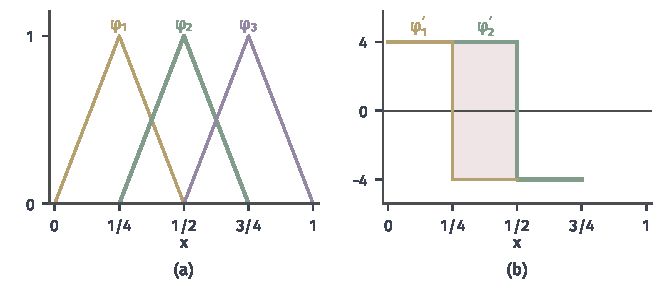
\includegraphics[width=112mm]{figures/06-differential-equations/02-partial-differential-equations/matplotlib/pdenum-hat-derivatives/figure.pdf}
 \caption{$h=1/4$的帽函数。(a)$\varphi_1,\varphi_2,\varphi_3$，相邻的帽函数才有公共支撑。(b)导数是分段常数，浅红区间是$\varphi_1'$（黄）与$\varphi_2'$（绿）唯一同时非零的区间，其上乘积为$-16$，积分得$K_{12}=-4$。}
 \label{fig:pdenum-hat-derivatives}
\end{BookInlineFigure}

每个积分都可以拆成单元上的积分之和，这把计算组织成了逐单元的循环。对单元$e=[x_{p},x_{q}]$，长度$h_e$，单元上只有$\varphi_p$和$\varphi_q$非零，它们的导数是$\mp1/h_e$，所以$2\times2$的\term{单元刚度矩阵}（element stiffness matrix）和单元载荷向量是
\begin{equation}
 \bm{k}^{e}=\frac{1}{h_e}\begin{bmatrix}1&-1\\-1&1\end{bmatrix},\qquad
 \bm{b}^{e}=\begin{bmatrix}\int_ef\varphi_p\,\mathrm{d}x\\\int_ef\varphi_q\,\mathrm{d}x\end{bmatrix}.
 \label{eq:pdenum-element-matrix}
\end{equation}
把它们按全局编号$p,q$累加到$\bm{K}$和$\bm{b}$中，这个过程称为\term{组装}（assembly）。

\needspace{6\baselineskip}
\paragraph{变量}
\begin{itemize}
 \item 节点数组$x_0,\ldots,x_n$，单元表：第$e$个单元的两个全局节点编号$(p_e,q_e)$。
 \item $\bm{K}\in\mathbb{R}^{(n+1)\times(n+1)}$：全局稀疏矩阵；$\bm{b}\in\mathbb{R}^{n+1}$：全局载荷。
 \item $\bm{k}^{e}\in\mathbb{R}^{2\times2}$，$\bm{b}^{e}\in\mathbb{R}^2$：当前单元的贡献。
\end{itemize}

\paragraph{初始化}
令$\bm{K}=\bm{0}$，$\bm{b}=\bm{0}$。例中$n=4$，$h_e=1/4$，$f=\pi^2\sin(\pi x)$，单元表为$(0,1),(1,2),(2,3),(3,4)$，节点从$0$编号。

\needspace{6\baselineskip}
\paragraph{每轮更新}
对每个单元执行下面三步，全部单元处理完后结束组装。
\begin{enumerate}
 \item 由式~\eqref{eq:pdenum-element-matrix}算出$\bm{k}^{e}$和$\bm{b}^{e}$。例中四个单元的$\bm{k}^{e}$相同，$1/h_e=4$。载荷用精确积分，四个单元依次是
 \[
  \begin{aligned}
  \bm{b}^{1}&=(0.3132,\,0.6070)^\top, & \bm{b}^{2}&=(1.0499,\,1.1716)^\top,\\
  \bm{b}^{3}&=(1.1716,\,1.0499)^\top, & \bm{b}^{4}&=(0.6070,\,0.3132)^\top.
  \end{aligned}
 \]
 \item 把$\bm{k}^{e}$加到$\bm{K}$的行列$(p_e,q_e)$上。例中第一轮后节点$0,1$构成的块是$4$乘以图~\ref{fig:pdenum-assembly}(a)的元素；第二轮再加到节点$1,2$的行列上，节点$1$的对角元变成$4+4=8$。图~\ref{fig:pdenum-assembly}是四轮的累加过程。
 \item 把$\bm{b}^{e}$加到$\bm{b}$的$p_e,q_e$分量上。例中内部节点的载荷累积成
 \[
  b_1=0.6070+1.0499=1.6569,\quad b_2=2\times1.1716=2.3431,\quad b_3=1.6569.
 \]
\end{enumerate}

\begin{BookInlineFigure}
 \centering
 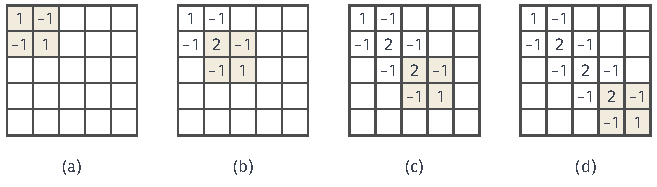
\includegraphics[width=112mm]{figures/06-differential-equations/02-partial-differential-equations/tikz/pdenum-assembly/figure.pdf}
 \caption{$n=4$的刚度矩阵（以$1/h$为单位）累加四个单元的贡献。(a)—(d)依次是加入第$1$到第$4$个单元后的结果，黄底是这一轮新加入的位置，重叠处的$1+1=2$来自相邻单元共享节点。方格是矩阵元素。}
 \label{fig:pdenum-assembly}
\end{BookInlineFigure}

组装结束后处理边值。例中$u(0)=0$、$u(1)=1$，节点$3$与边界节点$4$的耦合是$K_{34}=-4$。按式~\eqref{eq:pdenum-lifted-system}，$-K_{34}g_4=+4$加在第三个方程上，内部系统为
\[
 4\begin{bmatrix}2&-1&0\\-1&2&-1\\0&-1&2\end{bmatrix}\bm{c}
 =\begin{bmatrix}1.6569\\2.3431\\5.6569\end{bmatrix}.
\]
用式~\eqref{eq:pdenum-thomas-forward}和式~\eqref{eq:pdenum-thomas-back}解这个三对角方程，最终得到
\[
 \bm{c}=(0.9571,\,1.5000,\,1.4571)^\top .
\]

这三个数正好是真解的节点值，这不是巧合。

\paragraph{节点精确性}
节点上没有误差，是因为此时节点处的Green函数恰好落在$V_h$里。

\begin{theorem}[一维节点精确]
 \label{thm:pdenum-nodal-exact}
 设$a(u,v)=\int_0^1u'v'\,\mathrm{d}x$，$V=H^1_0(0,1)$，$V_h$是任意网格上的分片线性函数空间，$u_h$是载荷精确积分的Galerkin解。则$u_h(x_i)=u(x_i)$对所有节点成立。
\end{theorem}

\begin{proof}
 固定内部节点$x_i$，取Green函数$G_i$：它在$[0,x_i]$和$[x_i,1]$上都是线性函数，$G_i(0)=G_i(1)=0$，且$a(w,G_i)=w(x_i)$对所有$w\in V$成立。$G_i$只在$x_i$处有折角，所以$G_i\in V_h$。

 在Galerkin正交性~\eqref{eq:pdenum-orthogonality}中取$v_h=G_i$，得
 \[
  u(x_i)-u_h(x_i)=a(u-u_h,G_i)=0 .
 \]
\end{proof}

这是一维常系数问题的特殊性质。二维的Green函数在节点处奇异，变系数问题的Green函数在单元内也不是线性的，节点精确都不再成立。

它却让载荷的积分误差可以单独看出来。若单元载荷用梯形公式，则$b_i\approx hf(x_i)$，方程组除以$h$后正是差分方程~\eqref{eq:pdenum-three-point}，解就是$(0.9946,1.5530,1.4946)$。这里的误差$0.0530$完全来自数值积分。

\paragraph{高维的组装}
二维时把区域分成三角形，$\varphi_i$是在节点$i$处为$1$、在其他节点处为$0$的分片线性函数，形如金字塔，支撑是围绕节点$i$的那些三角形（图~\ref{fig:pdenum-triangle-mesh}(a)）。组装的循环完全不变，只是单元矩阵变成$3\times3$。梯度在三角形上是常向量，所以
\begin{equation}
 k^{e}_{ab}=\lvert e\rvert\,\nabla\varphi_a\cdot\nabla\varphi_b .
 \label{eq:pdenum-triangle-matrix}
\end{equation}

\begin{BookInlineFigure}
 \centering
 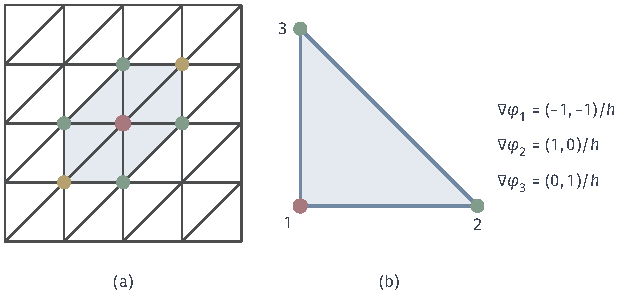
\includegraphics[width=106mm]{figures/06-differential-equations/02-partial-differential-equations/tikz/pdenum-triangle-mesh/figure.pdf}
 \caption{(a)规则三角网格，浅蓝区域是红点处基函数的支撑，由六个三角形组成，绿点和黄点是有公共单元的邻点。(b)直角边长$h$的三角形单元，三个基函数的梯度列在右侧。}
 \label{fig:pdenum-triangle-mesh}
\end{BookInlineFigure}

对图~\ref{fig:pdenum-triangle-mesh}(b)的直角三角形，$\lvert e\rvert=h^2/2$，由式~\eqref{eq:pdenum-triangle-matrix}得
\[
 \bm{k}^{e}=\frac12\begin{bmatrix}2&-1&-1\\-1&1&0\\-1&0&1\end{bmatrix}.
\]
$h$约掉了，二维的刚度矩阵元素与单元大小无关。

把中心节点周围六个三角形的贡献加起来。两个三角形的直角顶点在中心，各贡献$1$，另外四个三角形的中心节点在锐角顶点，各贡献$1/2$，对角元是$4$。四个水平、竖直邻点的边各被两个三角形共享，每个贡献$-1/2$，非对角元是$-1$；两个黄色邻点对应的矩阵元是$0$。这正是五点公式~\eqref{eq:pdenum-five-point}的模板。有限元的好处是，不规则的网格也可以用同样的循环组装。

\paragraph{各自保留的误差来源}
实际计算与上面的理想情形还有三处不同。载荷和变系数的积分通常用数值积分代替，这时解的是一个扰动后的方程，它的误差不包含在下一小节的估计里。

边界弯曲时，多边形网格覆盖的区域与真实区域不同，$V_h$可能不再是$V$的子空间，协调性被破坏，需要曲边单元或额外的分析。最后，线性方程组是用有限精度算出来的，残差不为零，Galerkin正交性也只是近似成立。

\subsection{逼近误差}
\label{sec:pdenum-fem-error}

$u_h$离$u$有多远？回答分成两步，第一步把问题化成纯粹的逼近问题，第二步才用到网格和解的光滑性。

\begin{theorem}[Céa估计]
 \label{thm:pdenum-cea}
 设$a$在$V$上有界且强制，常数分别为$M$和$\alpha$，$V_h\subset V$，$u$和$u_h$分别满足式~\eqref{eq:pdenum-weak}和式~\eqref{eq:pdenum-galerkin}。则
 \begin{equation}
  \lVert u-u_h\rVert_V\leq\frac{M}{\alpha}\inf_{v_h\in V_h}\lVert u-v_h\rVert_V .
  \label{eq:pdenum-cea}
 \end{equation}
\end{theorem}

\begin{proof}
 记$e=u-u_h$，取任意$v_h\in V_h$。由强制性，
 \[
  \alpha\lVert e\rVert_V^2\leq a(e,e) .
 \]
 把第二个$e$写成$(u-v_h)+(v_h-u_h)$，其中$v_h-u_h\in V_h$，由式~\eqref{eq:pdenum-orthogonality}，这一部分的贡献为零：
 \[
  a(e,e)=a(e,u-v_h) .
 \]
 由有界性，
 \[
  a(e,u-v_h)\leq M\lVert e\rVert_V\lVert u-v_h\rVert_V .
 \]
 三式相连，约去$\lVert e\rVert_V$（$e=0$时结论已成立），再对$v_h$取下确界。
\end{proof}

三个条件各有作用。有界性和强制性给出常数比$M/\alpha$，它描述问题的条件好坏；协调性让Galerkin正交性可用。$a$对称时，在能量范数$\lVert v\rVert_a=a(v,v)^{1/2}$下常数是$1$，$u_h$就是能量范数下的最佳逼近。

定理只说$u_h$不比$V_h$中最好的函数差多少。第二步要估计$V_h$的逼近能力，常用的办法是取节点插值$I_hu$作为具体的候选。

\begin{lemma}[分片线性插值误差]
 \label{lem:pdenum-interpolation}
 设$u\in H^2(0,1)$，$I_hu$是$u$在最大步长为$h$的网格上的分片线性插值，则
 \begin{equation}
  \lVert(u-I_hu)'\rVert_{L^2}\leq\frac{h}{\pi}\lVert u''\rVert_{L^2} .
  \label{eq:pdenum-interpolation}
 \end{equation}
\end{lemma}

\begin{proof}
 在一个单元$[a,b]$上，长度$\ell\leq h$，记$e=u-I_hu$。$e(a)=e(b)=0$，所以$\int_a^be'\,\mathrm{d}x=0$，即$e'$的平均为零。

 把$e'$按余弦函数$\cos(k\pi(x-a)/\ell)$展开，平均为零使$k=0$的项消失，系数记为$c_k$。由Parseval恒等式，
 \[
  \int_a^b(e')^2\,\mathrm{d}x=\frac{\ell}{2}\sum_{k\geq1}c_k^2\leq\frac{\ell^2}{\pi^2}\cdot\frac{\ell}{2}\sum_{k\geq1}\Bigl(\frac{k\pi}{\ell}\Bigr)^2c_k^2=\frac{\ell^2}{\pi^2}\int_a^b(e'')^2\,\mathrm{d}x .
 \]
 单元内$I_hu$线性，所以$e''=u''$。对所有单元求和即得结论。
\end{proof}

合并Céa估计与引理。在一维Poisson问题上，$a$对称，常数是$1$，能量误差满足
\begin{equation}
 \lVert(u-u_h)'\rVert_{L^2}\leq\frac{h}{\pi}\lVert u''\rVert_{L^2} .
 \label{eq:pdenum-energy-rate}
\end{equation}

$L^2$范数下的误差比能量范数高一阶，这要用到对偶论证。

\begin{theorem}[$L^2$误差]
 \label{thm:pdenum-l2}
 在一维Poisson问题上，若$u\in H^2(0,1)$，则
 \begin{equation}
  \lVert u-u_h\rVert_{L^2}\leq\frac{h}{\pi}\lVert(u-u_h)'\rVert_{L^2}\leq\frac{h^2}{\pi^2}\lVert u''\rVert_{L^2} .
  \label{eq:pdenum-l2-rate}
 \end{equation}
\end{theorem}

\begin{proof}
 记$e=u-u_h$，$z$是对偶问题$-z''=e$，$z(0)=z(1)=0$的解，$z\in H^2$且$\lVert z''\rVert_{L^2}=\lVert e\rVert_{L^2}$。用$e$检验对偶问题并分部积分，
 \[
  \lVert e\rVert_{L^2}^2=a(e,z) .
 \]
 由Galerkin正交性可以减去$I_hz\in V_h$：
 \[
  a(e,z)=a(e,z-I_hz)\leq\lVert e'\rVert_{L^2}\lVert(z-I_hz)'\rVert_{L^2} .
 \]
 用引理~\ref{lem:pdenum-interpolation}估计第二个因子，并用$\lVert z''\rVert_{L^2}=\lVert e\rVert_{L^2}$，得到
 \[
  \lVert e\rVert_{L^2}^2\leq\frac{h}{\pi}\lVert e'\rVert_{L^2}\lVert e\rVert_{L^2} .
 \]
 约去$\lVert e\rVert_{L^2}$，得第一个不等式；第二个不等式由式~\eqref{eq:pdenum-energy-rate}得到。
\end{proof}

例中$\lVert u''\rVert_{L^2}=\pi^2/\sqrt2\approx6.979$。$h=1/4$时，能量误差的上界是$0.5554$，实际是$0.4985$；$L^2$误差的中间上界是$(h/\pi)\times0.4985=0.0397$，实际是$0.0393$。$h=1/8$时对应的四个数是$0.2777$、$0.2512$、$0.0100$、$0.0099$。

\paragraph{实际阶数还看什么}
式~\eqref{eq:pdenum-energy-rate}要求$u\in H^2$。把解换成$u=x^{3/4}-x$，它属于$H^1_0$，$u''$却不平方可积。由定理~\ref{thm:pdenum-nodal-exact}，这时$u_h$就是节点插值，能量误差可以用积分精确算出。图~\ref{fig:pdenum-fem-rates}(b)表明，均匀网格的观测阶只有$0.25$。

\begin{BookInlineFigure}
 \centering
 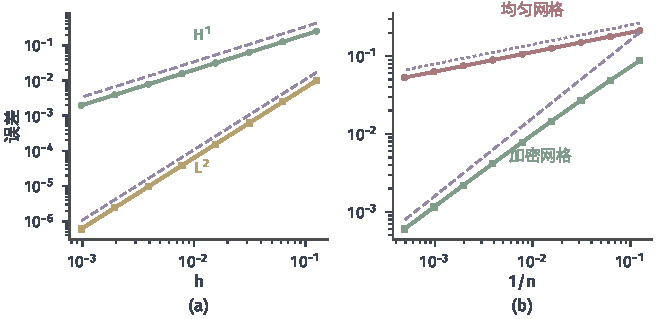
\includegraphics[width=112mm]{figures/06-differential-equations/02-partial-differential-equations/matplotlib/pdenum-fem-rates/figure.pdf}
 \caption{分片线性元的误差，紫线是参考斜率。(a)光滑解$\sin(\pi x)+x$：绿线$H^1$半范数，斜率$1$；黄线$L^2$范数，斜率$2$。(b)$u=x^{3/4}-x$的$H^1$半范数：红线是均匀网格，斜率$0.25$；绿线是向$0$加密的网格$x_i=(i/n)^4$，斜率接近$1$。}
 \label{fig:pdenum-fem-rates}
\end{BookInlineFigure}

问题集中在$x=0$附近，解的导数在那里无界。把节点按$x_i=(i/n)^4$向$0$加密后，单元数目不变，观测阶从$0.83$逐渐升到$0.94$，接近一阶。收敛阶不是方法的固有性质，它还取决于解的正则性和网格是否与之匹配。

高维的情形要结合更多因素。$k$次单元在解足够光滑、网格形状规则（三角形不退化）时，$H^1$误差是$O(h^k)$，$L^2$误差是$O(h^{k+1})$，后者还要求对偶问题具有$H^2$正则性。严格的证明需要Bramble--Hilbert引理和单元上的尺度变换，篇幅较长，读者可查阅有限元方法的专著。非凸多边形的角点附近解不属于$H^2$，均匀网格上的阶数会下降，机制与上面的一维例子相同。
